\documentclass[12pt]{article}
\usepackage[utf8]{inputenc}
\usepackage[english]{babel}

\usepackage[letterpaper, margin = 1in]{geometry}
\usepackage{verbatim}
\usepackage{fancyhdr}
\usepackage{titling}
\usepackage{titlesec }
\usepackage{hyperref}
\usepackage{setspace}
\usepackage{hanging}
\usepackage{tree-dvips}
\usepackage{tikz}
\usepackage{gb4e}


\title{theory}
\author{Databook}
\date{}


\pagestyle{fancy}

\widowpenalty=100000
\clubpenalty=100000

\titleformat*{\section}{\medium\bfseries}
\titleformat*{\subsection}{\medium\bfseries}
\titleformat*{\subsubsection}{\medium\bfseries}

\begin{document}

\pagestyle{empty}

\section*{Theorist Quads}\par

\centering

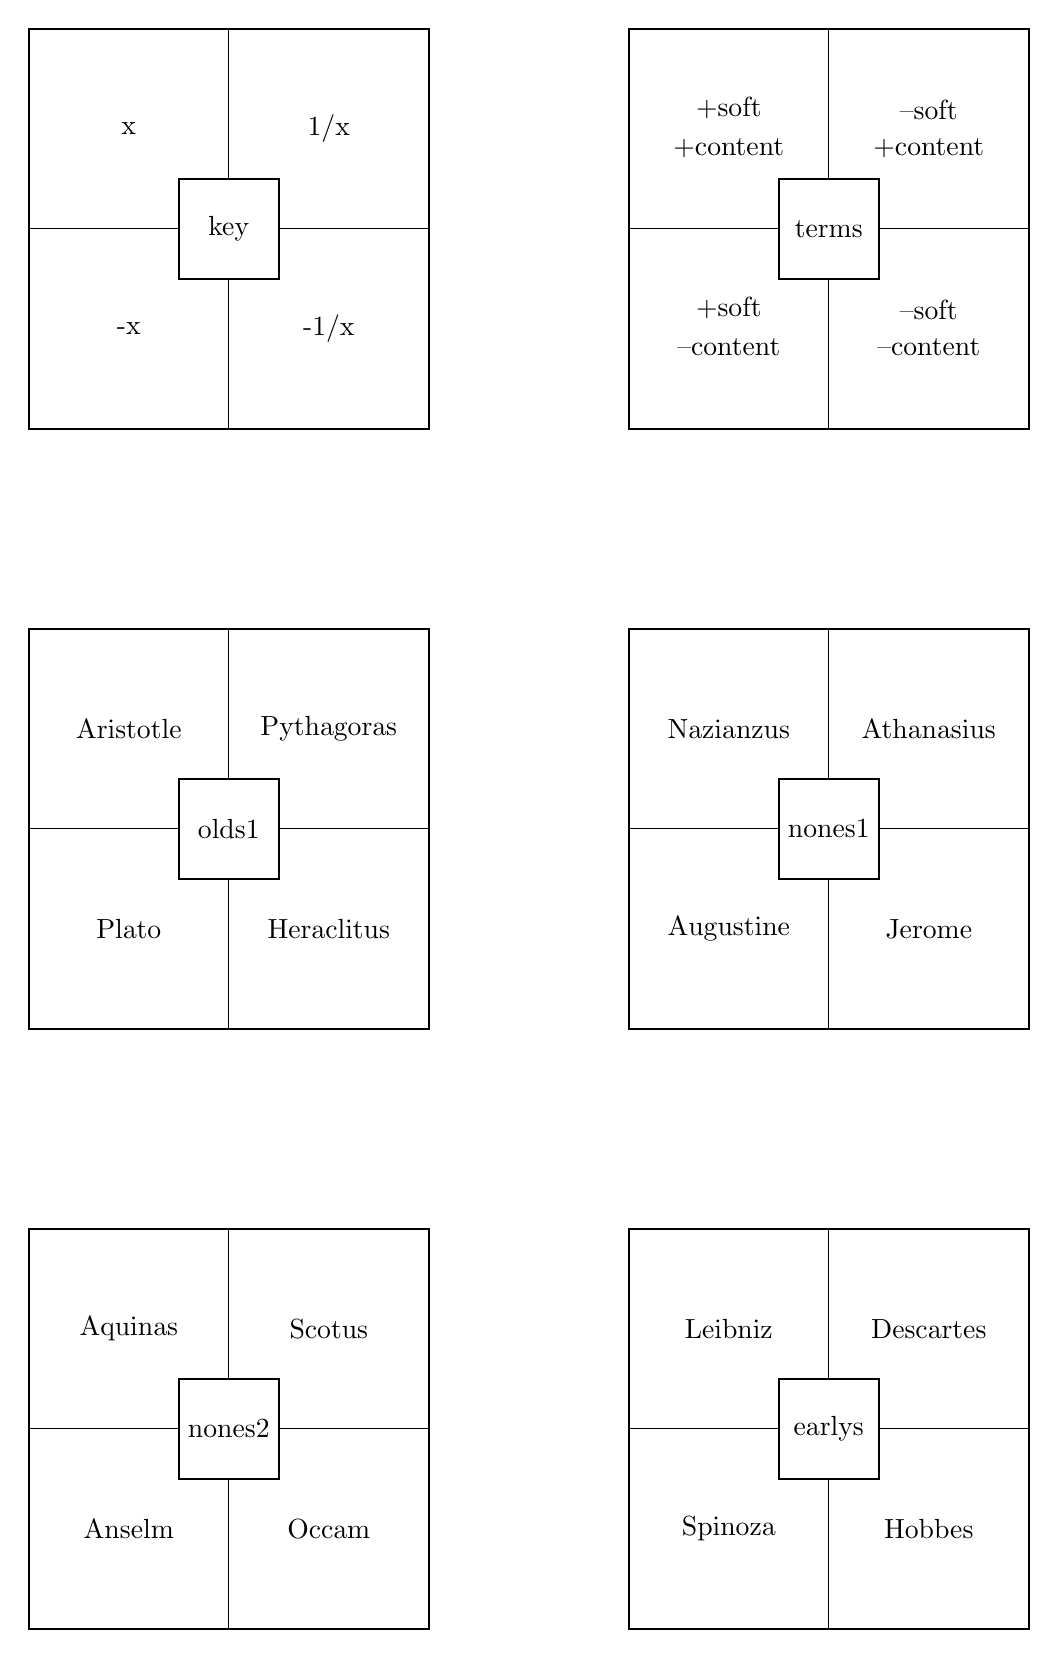
\begin{tikzpicture} [x=1in,y=1in]

%\draw [step=1in, dotted, thick] (0,0) grid (6,8);

\draw [thick] (0.5,6) rectangle (2.5,8);
\draw [thick] (1.25,6.75) rectangle (1.75,7.25);
\draw (0.5,7) -- (1.25,7);
\draw (1.75,7) -- (2.5,7);
\draw (1.5,6) -- (1.5,6.75);
\draw (1.5,7.25) -- (1.5,8);
\node at (1.5,7) {key};
\node at (1,7.5) {x};
\node at (2,7.5) {1/x};
\node at (1,6.5) {-x};
\node at (2,6.5) {-1/x};

\draw [thick] (3.5,6) rectangle (5.5,8);
\draw [thick] (4.25,6.75) rectangle (4.75,7.25);
\draw (3.5,7) -- (4.25,7);
\draw (4.75,7) -- (5.5,7);
\draw (4.5,6) -- (4.5,6.75);
\draw (4.5,7.25) -- (4.5,8);
\node at (4.5,7) {terms};
\node [above] at (4,7.5) {+soft};
\node [below] at (4,7.5) {+content};
\node [above] at (5,7.5) {--soft};
\node [below] at (5,7.5) {+content};
\node [above] at (4,6.5) {+soft};
\node [below] at (4,6.5) {--content};
\node [above] at (5,6.5) {--soft};
\node [below] at (5,6.5) {--content};

\draw [thick] (0.5,3) rectangle (2.5,5);
\draw [thick] (1.25,3.75) rectangle (1.75,4.25);
\draw (0.5,4) -- (1.25,4);
\draw (1.75,4) -- (2.5,4);
\draw (1.5,3) -- (1.5,3.75);
\draw (1.5,4.25) -- (1.5,5);
\node at (1.5,4) {olds1};
\node at (1,4.5) {Aristotle};
\node at (2,4.5) {Pythagoras};
\node at (1,3.5) {Plato};
\node at (2,3.5) {Heraclitus};

\draw [thick] (3.5,3) rectangle (5.5,5);
\draw [thick] (4.25,3.75) rectangle (4.75,4.25);
\draw (3.5,4) -- (4.25,4);
\draw (4.75,4) -- (5.5,4);
\draw (4.5,3) -- (4.5,3.75);
\draw (4.5,4.25) -- (4.5,5);
\node at (4.5,4) {nones1};
\node at (4,4.5) {Nazianzus};
\node at (5,4.5) {Athanasius};
\node at (4,3.5) {Augustine};
\node at (5,3.5) {Jerome};

\draw [thick] (0.5,0) rectangle (2.5,2);
\draw [thick] (1.25,0.75) rectangle (1.75,1.25);
\draw (0.5,1) -- (1.25,1);
\draw (1.75,1) -- (2.5,1);
\draw (1.5,0) -- (1.5,0.75);
\draw (1.5,1.25) -- (1.5,2);
\node at (1.5,1) {nones2};
\node at (1,1.5) {Aquinas};
\node at (2,1.5) {Scotus};          
\node at (1,0.5) {Anselm};
\node at (2,0.5) {Occam};

\draw [thick] (3.5,0) rectangle (5.5,2);
\draw [thick] (4.25,0.75) rectangle (4.75,1.25);
\draw (3.5,1) -- (4.25,1);
\draw (4.75,1) -- (5.5,1);
\draw (4.5,0) -- (4.5,0.75);
\draw (4.5,1.25) -- (4.5,2);
\node at (4.5,1) {earlys};
\node at (4,1.5) {Leibniz};
\node at (5,1.5) {Descartes};
\node at (4,0.5) {Spinoza};
\node at (5,0.5) {Hobbes};

\end{tikzpicture}

\newpage

\pagestyle{empty}

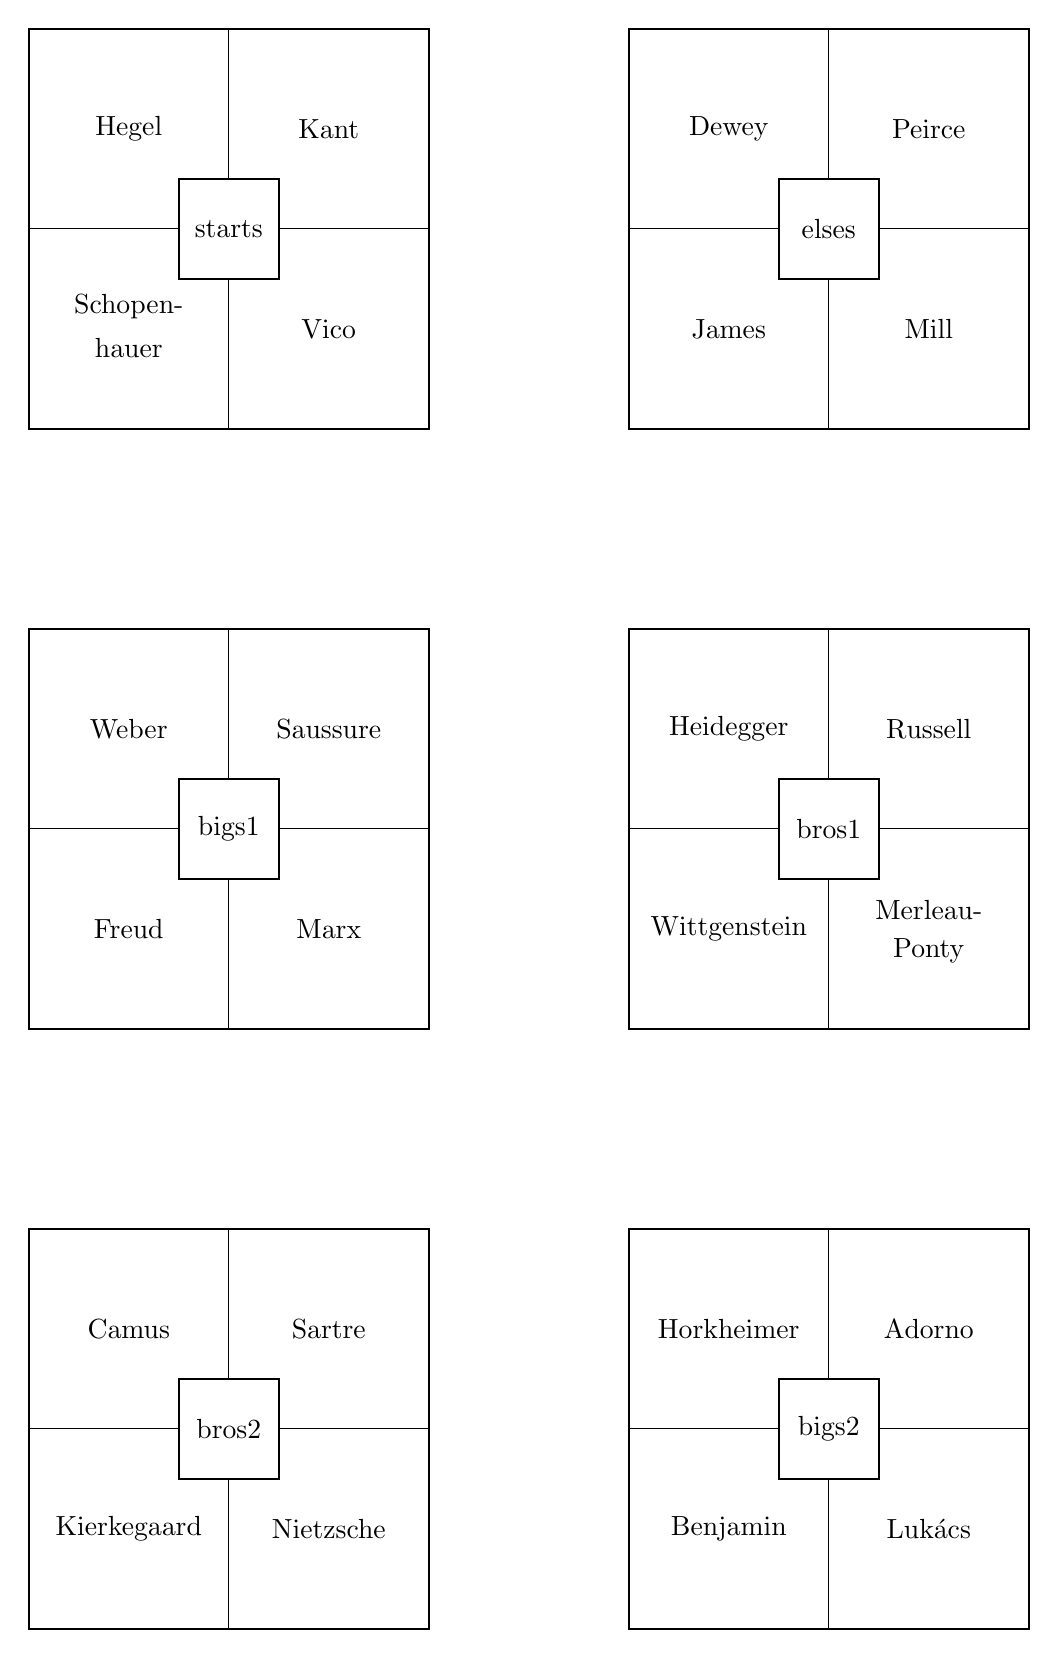
\begin{tikzpicture} [x=1in,y=1in]

%\draw [step=1in, dotted, thick] (0,0) grid (6,8);

\draw [thick] (0.5,6) rectangle (2.5,8);
\draw [thick] (1.25,6.75) rectangle (1.75,7.25);
\draw (0.5,7) -- (1.25,7);
\draw (1.75,7) -- (2.5,7);
\draw (1.5,6) -- (1.5,6.75);
\draw (1.5,7.25) -- (1.5,8);
\node at (1.5,7) {starts};
\node at (1,7.5) {Hegel};
\node at (2,7.5) {Kant};
\node [above] at (1,6.5) {Schopen-};
\node [below] at (1,6.5) {hauer};
\node at (2,6.5) {Vico};

\draw [thick] (3.5,6) rectangle (5.5,8);
\draw [thick] (4.25,6.75) rectangle (4.75,7.25);
\draw (3.5,7) -- (4.25,7);
\draw (4.75,7) -- (5.5,7);
\draw (4.5,6) -- (4.5,6.75);
\draw (4.5,7.25) -- (4.5,8);
\node at (4.5,7) {elses};
\node at (4,7.5) {Dewey};
\node at (5,7.5) {Peirce};
\node at (4,6.5) {James};
\node at (5,6.5) {Mill};

\draw [thick] (0.5,3) rectangle (2.5,5);
\draw [thick] (1.25,3.75) rectangle (1.75,4.25);
\draw (0.5,4) -- (1.25,4);
\draw (1.75,4) -- (2.5,4);
\draw (1.5,3) -- (1.5,3.75);
\draw (1.5,4.25) -- (1.5,5);
\node at (1.5,4) {bigs1};
\node at (1,4.5) {Weber};
\node at (2,4.5) {Saussure};
\node at (1,3.5) {Freud};
\node at (2,3.5) {Marx};

\draw [thick] (3.5,3) rectangle (5.5,5);
\draw [thick] (4.25,3.75) rectangle (4.75,4.25);
\draw (3.5,4) -- (4.25,4);
\draw (4.75,4) -- (5.5,4);
\draw (4.5,3) -- (4.5,3.75);
\draw (4.5,4.25) -- (4.5,5);
\node at (4.5,4) {bros1};
\node at (4,4.5) {Heidegger};
\node at (5,4.5) {Russell};
\node at (4,3.5) {Wittgenstein};
\node [above] at (5,3.5) {Merleau-};
\node [below] at (5,3.5) {Ponty};

\draw [thick] (0.5,0) rectangle (2.5,2);
\draw [thick] (1.25,0.75) rectangle (1.75,1.25);
\draw (0.5,1) -- (1.25,1);
\draw (1.75,1) -- (2.5,1);
\draw (1.5,0) -- (1.5,0.75);
\draw (1.5,1.25) -- (1.5,2);
\node at (1.5,1) {bros2};
\node at (1,1.5) {Camus};
\node at (2,1.5) {Sartre};
\node at (1,0.5) {Kierkegaard};
\node at (2,0.5) {Nietzsche};

\draw [thick] (3.5,0) rectangle (5.5,2);
\draw [thick] (4.25,0.75) rectangle (4.75,1.25);
\draw (3.5,1) -- (4.25,1);
\draw (4.75,1) -- (5.5,1);
\draw (4.5,0) -- (4.5,0.75);
\draw (4.5,1.25) -- (4.5,2);
\node at (4.5,1) {bigs2};
\node at (4,1.5) {Horkheimer};
\node at (5,1.5) {Adorno};
\node at (4,0.5) {Benjamin};
\node at (5,0.5) {Luk\'{a}cs};

\end{tikzpicture}

\newpage

\pagestyle{empty}

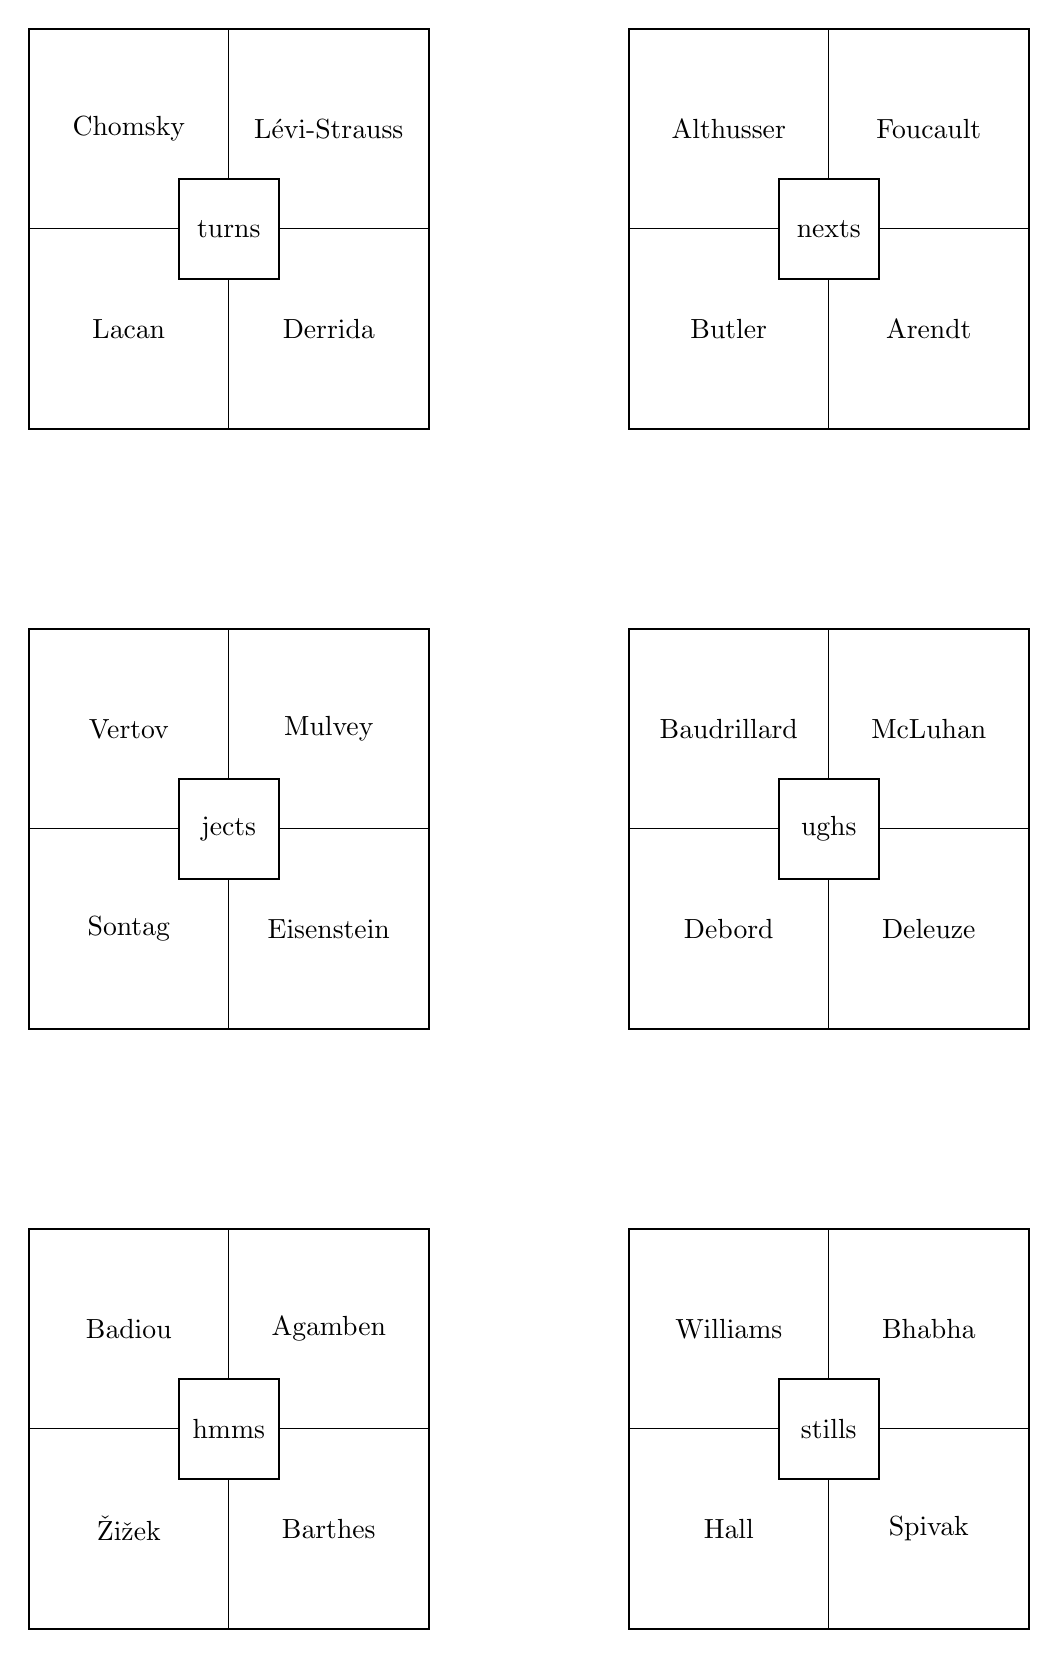
\begin{tikzpicture} [x=1in,y=1in]

%\draw [step=1in, dotted, thick] (0,0) grid (6,8);

\draw [thick] (0.5,6) rectangle (2.5,8);
\draw [thick] (1.25,6.75) rectangle (1.75,7.25);
\draw (0.5,7) -- (1.25,7);
\draw (1.75,7) -- (2.5,7);
\draw (1.5,6) -- (1.5,6.75);
\draw (1.5,7.25) -- (1.5,8);
\node at (1.5,7) {turns};
\node at (1,7.5) {Chomsky};
\node at (2,7.5) {L\'{e}vi-Strauss};
\node at (1,6.5) {Lacan};
\node at (2,6.5) {Derrida};

\draw [thick] (3.5,6) rectangle (5.5,8);
\draw [thick] (4.25,6.75) rectangle (4.75,7.25);
\draw (3.5,7) -- (4.25,7);
\draw (4.75,7) -- (5.5,7);
\draw (4.5,6) -- (4.5,6.75);
\draw (4.5,7.25) -- (4.5,8);
\node at (4.5,7) {nexts};
\node at (4,7.5) {Althusser};
\node at (5,7.5) {Foucault};
\node at (4,6.5) {Butler};
\node at (5,6.5) {Arendt};

\draw [thick] (0.5,3) rectangle (2.5,5);
\draw [thick] (1.25,3.75) rectangle (1.75,4.25);
\draw (0.5,4) -- (1.25,4);
\draw (1.75,4) -- (2.5,4);
\draw (1.5,3) -- (1.5,3.75);
\draw (1.5,4.25) -- (1.5,5);
\node at (1.5,4) {jects};
\node at (1,4.5) {Vertov};
\node at (2,4.5) {Mulvey};
\node at (1,3.5) {Sontag};
\node at (2,3.5) {Eisenstein};

\draw [thick] (3.5,3) rectangle (5.5,5);
\draw [thick] (4.25,3.75) rectangle (4.75,4.25);
\draw (3.5,4) -- (4.25,4);
\draw (4.75,4) -- (5.5,4);
\draw (4.5,3) -- (4.5,3.75);
\draw (4.5,4.25) -- (4.5,5);
\node at (4.5,4) {ughs};
\node at (4,4.5) {Baudrillard};
\node at (5,4.5) {McLuhan};
\node at (4,3.5) {Debord};
\node at (5,3.5) {Deleuze};

\draw [thick] (0.5,0) rectangle (2.5,2);
\draw [thick] (1.25,0.75) rectangle (1.75,1.25);
\draw (0.5,1) -- (1.25,1);
\draw (1.75,1) -- (2.5,1);
\draw (1.5,0) -- (1.5,0.75);
\draw (1.5,1.25) -- (1.5,2);
\node at (1.5,1) {hmms};
\node at (1,1.5) {Badiou};
\node at (2,1.5) {Agamben};
\node at (1,0.5) {\v{Z}i\v{z}ek};
\node at (2,0.5) {Barthes};

\draw [thick] (3.5,0) rectangle (5.5,2);
\draw [thick] (4.25,0.75) rectangle (4.75,1.25);
\draw (3.5,1) -- (4.25,1);
\draw (4.75,1) -- (5.5,1);
\draw (4.5,0) -- (4.5,0.75);
\draw (4.5,1.25) -- (4.5,2);
\node at (4.5,1) {stills};
\node at (4,1.5) {Williams};
\node at (5,1.5) {Bhabha};
\node at (4,0.5) {Hall};
\node at (5,0.5) {Spivak};

\end{tikzpicture}

\end{document}